\section{Advanced Classification}
\label{sec:advanced_classification}

In this section, classification results are showcased for two
target variables: \texttt{averageRating} (properly binned into
5 classes), and \texttt{titleType} (with 6 classes).

\textcolor{red}{We then applied multiple classification models using the data as preprocessed previously (see Section~\ref{sec:understanding_preparation}).}   
\textcolor{blue}{The first target variable is \texttt{titleType}, which includes six categories: 
\textit{movie}, \textit{short}, \textit{tvEpisode}, \textit{tvSeries}, 
\textit{tvSpecial}, and \textit{video}. 
The classes are not equally distributed, with \textit{tvSpecial} and \textit{video} 
being significantly under-represented compared to the others. Entries labeled as \textit{videoGame} were removed from both the training and testing sets, 
as they were too few to be useful for classification. 
The remaining categories were merged into broader groups according to the following mapping: 
\textit{movie} and \textit{tvMovie} were grouped as \textit{movie}, 
\textit{short} and \textit{tvShort} were grouped as \textit{short}, 
\textit{tvSeries} and \textit{tvMiniSeries} were grouped as \textit{tvSeries}, 
while \textit{tvEpisode}, \textit{tvSpecial} and \textit{video} were left unchanged. 
All feature columns were standardized using a \textit{StandardScaler}. 
In addition, the variable \texttt{canHaveEpisodes} was removed prior to training, 
since it provides direct information about the target \texttt{titleType} 
and could therefore introduce data leakage.}

\subsection{Support Vector Machines}
\label{subsec:svm}

We applied Support Vector Machines (SVM) to the \texttt{titleType} classification task.
Both linear and non-linear kernels were explored in order to evaluate how decision boundary complexity influences predictive performance.

The first experiment used a Linear SVM trained on the full dataset.  
A grid search with five-fold cross validation was carried out on the parameters 
$C \in \{0.01, 0.1, 1, 10, 100\}$ and $max\_iter \in \{1000, 5000, 10000\}$. 
The optimal configuration, with $C=100$ and $max\_iter=1000$, achieved a test accuracy of 0.81. 
While precision and recall were high for majority classes (\textit{movie}, \textit{short}, \textit{tvEpisode}), 
the classifier failed on \textit{tvSeries}, \textit{tvSpecial}, and \textit{video}, 
indicating that a linear decision boundary is insufficient for this problem.  

Non-linear kernels were then evaluated. 
A grid search was first performed on a stratified 10\% subset of the training set to efficiently explore a wide range of hyperparameters for each kernel, 
since a full search on the complete dataset would have been computationally prohibitive. 
For the RBF kernel, $C$ was varied from 0.01 to 1000 and $\gamma$ between \texttt{scale} and \texttt{auto}. 
The polynomial kernel was tested with $C$ from 0.01 to 100, degree 2--4, $\gamma$ as \texttt{scale} or \texttt{auto}, and \texttt{coef0} 0 or 1. 
The sigmoid kernel was explored over $C$ 0.01--100, $\gamma$ \texttt{scale}/\texttt{auto}, and \texttt{coef0} 0 or 1. 
\textcolor{blue}{Remember to fix C!}

The best configuration for each kernel, reported in Table~\ref{tab:svm_results}, was then retrained on the full dataset and evaluated on the test set. 
Both RBF and polynomial kernels reached approximately 0.90 test accuracy, substantially outperforming the linear baseline and sigmoid. 
The RBF kernel was selected as the reference non-linear model due to slightly more stable results and improved recall on the under-represented classes.


ROC curves were used to evaluate class separability (Figure~\ref{fig:roc_four}),
showing excellent separation for majority classes, although minority categories remained problematic. 

\textcolor{red}{I will change the text and explain the figures better.}

To address class imbalance, the RBF kernel was retrained with \texttt{class\_weight=balanced}, 
which penalizes misclassification of under-represented classes. 
This model reached a slightly lower overall accuracy of 0.84, 
but recall for \textit{tvSpecial} and \textit{video} improved, providing a more equitable classification across categories.  
Confusion matrices (Figure~\ref{fig:rbf_balanced_two}) 
illustrate that \textit{tvSpecial} and \textit{video} ...  
Analysis of the support vectors confirmed this effect. 
In the unbalanced RBF, nearly all points of minority classes became support vectors, 
while in the balanced model the total number of support vectors increased and was more evenly distributed across classes, 
indicating a more complex but fairer decision function. 

Table~\ref{tab:svm_results} summarizes the main results, including the parameters used for each kernel and the corresponding test performance. 


\begin{table}[h]
\centering
\caption{Comparison of SVM models on the IMDb classification task.}
\label{tab:svm_results}
\begin{tabular}{lccc}
\hline
\textbf{Model} & \textbf{Best Params (main)} & \textbf{Test Accuracy} & \textbf{Macro F1-score} \\
\hline
Linear SVM & $C=100$, $max\_iter=1000$ & 0.81 & 0.45 \\
RBF kernel & $C=10$, $\gamma=\text{scale}$ & 0.90 & 0.64 \\
Polynomial kernel & $C=10$, degree=3, $\gamma=\text{auto}$ & 0.90 & 0.64 \\
Sigmoid kernel & $C=0.1$, $\gamma=\text{auto}$ & 0.65 & 0.36 \\
RBF (balanced) & $C=10$, $\gamma=\text{scale}$, balanced & 0.84 & 0.65 \\
\hline
\end{tabular}
\end{table}
    
% --- First figure: four ROC curves side by side ---
\begin{figure}[h]
    \centering
    \begin{subfigure}[b]{0.24\textwidth}
        \centering
        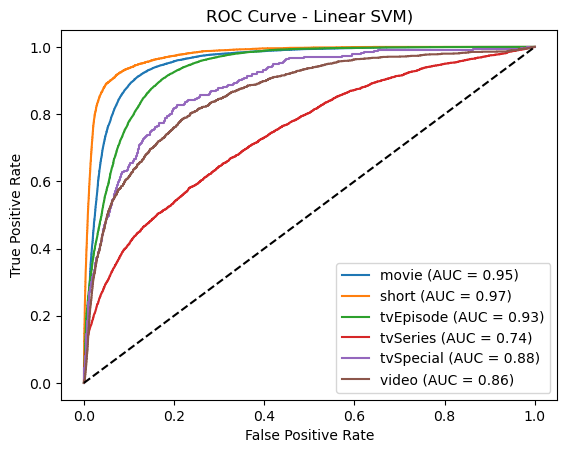
\includegraphics[width=\textwidth]{plotsss/roc_linear.png}
        \caption{Linear SVM}
        \label{fig:roc_linear}
    \end{subfigure}
    \begin{subfigure}[b]{0.24\textwidth}
        \centering
        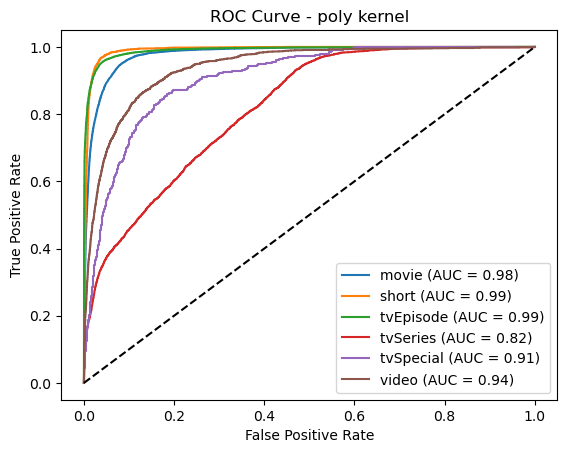
\includegraphics[width=\textwidth]{plotsss/roc_poly.png}
        \caption{Polynomial kernel}
        \label{fig:roc_poly}
    \end{subfigure}
    \begin{subfigure}[b]{0.24\textwidth}
        \centering
        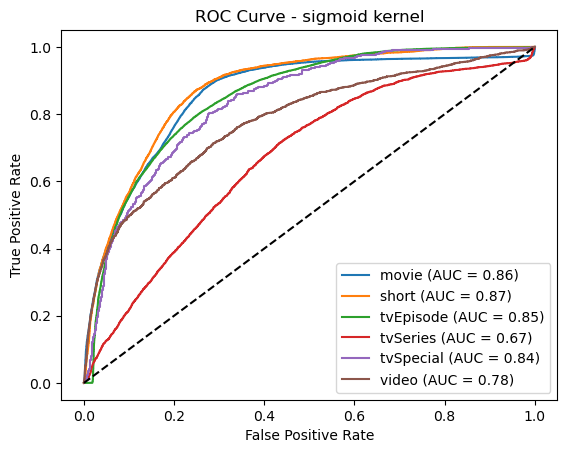
\includegraphics[width=\textwidth]{plotsss/roc_sigmoid.png}
        \caption{Sigmoid kernel}
        \label{fig:roc_sigmoid}
    \end{subfigure}
    \begin{subfigure}[b]{0.24\textwidth}
        \centering
        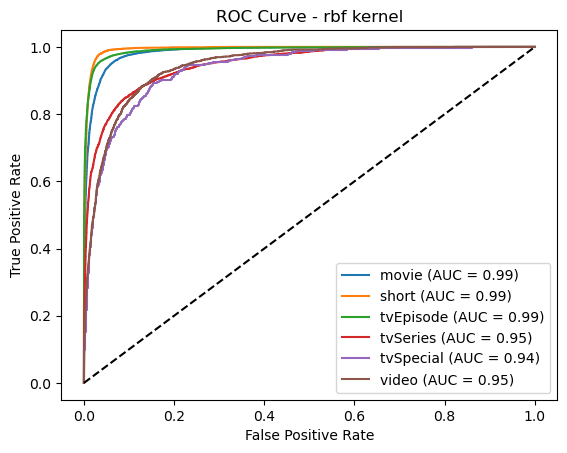
\includegraphics[width=\textwidth]{plotsss/roc_rbf.png}
        \caption{RBF kernel}
        \label{fig:roc_rbf}
    \end{subfigure}
    \caption{...}  
    \label{fig:roc_four}
\end{figure}

% --- Second figure: confusion matrix and ROC for RBF balanced ---
\begin{figure}[h]
    \centering
    \begin{subfigure}[b]{0.48\textwidth}
        \centering
        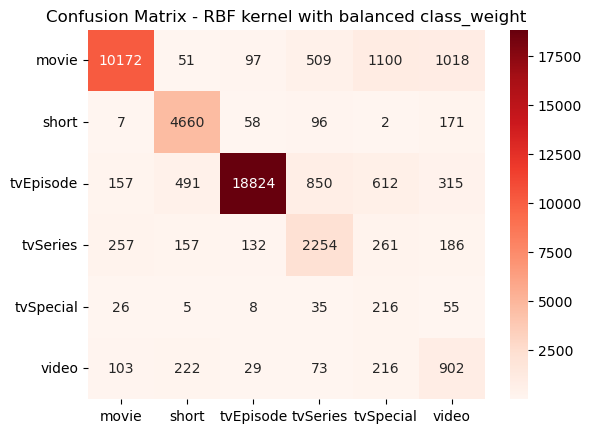
\includegraphics[width=\textwidth]{plotsss/cm_rbf_balanced.png}
        \caption{Confusion Matrix RBF balanced}
        \label{fig:cm_rbf_balanced}
    \end{subfigure}
    \begin{subfigure}[b]{0.48\textwidth}
        \centering
        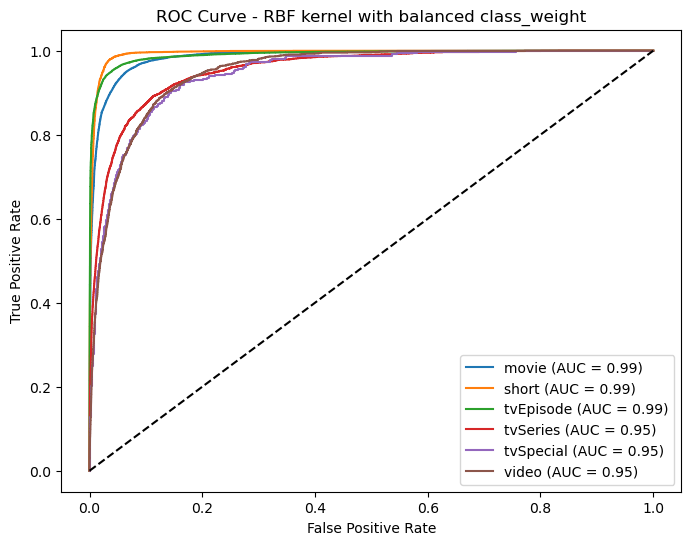
\includegraphics[width=\textwidth]{plotsss/roc_rbf_balanced.png}
        \caption{ROC RBF balanced}
        \label{fig:roc_rbf_balanced}
    \end{subfigure}
    \caption{...}  
    \label{fig:rbf_balanced_two}
\end{figure}

% In conclusion, non-linear kernels were clearly superior to the linear SVM, 
% with RBF and polynomial achieving comparable accuracy. 
% The RBF kernel with balanced class weights provided the best compromise, 
% maintaining strong performance on majority classes while improving recognition of minority ones.



\subsection{Ensemble methods}
Boosting and Random Forest models were trained on the classification,
while being optimized via Stratified Randomized Search with 5-fold
cross-validation over a predefined hyperparameter space.\\

% rf
% RandomForestClassifier(max_depth=19, max_features=0.7361716094628554,
                    %    min_samples_leaf=3, min_samples_split=4, n_estimators=42,
                    %    n_jobs=-1, random_state=42)
% precision    recall  f1-score   support

%            0       0.56      0.60      0.58      9717
%            1       0.44      0.34      0.39     11114
%            2       0.48      0.68      0.56     14674
%            3       0.46      0.27      0.34      7640
%            4       0.60      0.16      0.25      1715

%     accuracy                           0.49     44860
%    macro avg       0.51      0.41      0.42     44860
% weighted avg       0.49      0.49      0.47     44860


% adaboost
% best_params = {'estimator__max_depth': 10, 'estimator__min_samples_leaf': 16, 'estimator__min_samples_split': 16, 'learning_rate': 0.46606998421703594, 'n_estimators': 56}
% precision    recall  f1-score   support

%            0       0.48      0.40      0.43      9717
%            1       0.33      0.31      0.32     11114
%            2       0.42      0.55      0.47     14674
%            3       0.31      0.28      0.29      7640
%            4       0.44      0.11      0.18      1715

%     accuracy                           0.39     44860
%    macro avg       0.40      0.33      0.34     44860
% weighted avg       0.39      0.39      0.38     44860

For the \texttt{averageRating} classification task, the best
hyperparameters for the Random Forest model were:
\texttt{n\_estimators=42}, \texttt{max\_depth=19}, \texttt{min\_samples\_split=4},
\texttt{min\_samples\_leaf=3}, \texttt{max\_features=0.74},
\texttt{criterion='gini'}, \texttt{class\_weight=None}.

For the AdaBoost model, the best hyperparameters were:
\texttt{n\_estimators=56}, \texttt{learning\_rate=0.47},
\texttt{estimator\_\_max\_depth=10},
\texttt{estimator\_\_min\_samples\_split=16},
\texttt{estimator\_\_min\_samples\_leaf=16}.

The table below summarizes the classification report for both models.
\begin{table}[H]
    \centering
    \label{tab:classification_report}
    \begin{tabular}{lccccc}
    \hline
    \textbf{Model} & \textbf{Accuracy} & \textbf{Macro Precision} & \textbf{Macro Recall} & \textbf{Macro F1-score} \\
    \hline
    Random Forest & 0.49 & 0.51 & 0.41 & 0.42 \\
    AdaBoost & 0.39 & 0.40 & 0.33 & 0.34 \\
    \hline
    \end{tabular}
    \caption{Performances of the models on the \texttt{averageRating} classification task.}
\end{table}

The Random Forest model outperforms AdaBoost in all metrics.
The biggest difference is found in the recall.

Figure~\ref{fig:cm_rf} and Figure~\ref{fig:cm_ab} show the confusion matrices
for the models.
\begin{figure}[H]
    \centering
    \begin{subfigure}[b]{0.45\textwidth}
        \centering
        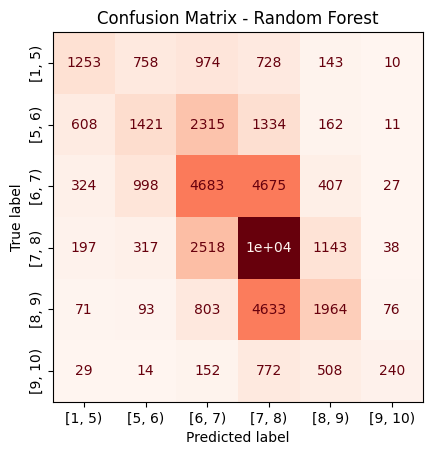
\includegraphics[width=\textwidth]{plotsss/conf_matr_rf_rating}
        \caption{Confusion Matrix - Random Forest}
        \label{fig:cm_rf}
    \end{subfigure}
    \hfill
    \begin{subfigure}[b]{0.45\textwidth}
        \centering
        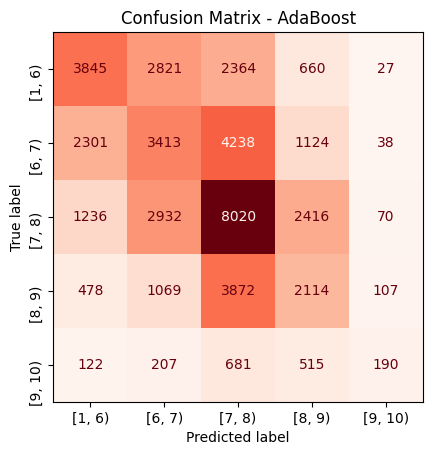
\includegraphics[width=\textwidth]{plotsss/conf_matr_boost_rating}
        \caption{Confusion Matrix - AdaBoost}
        \label{fig:cm_ab}
    \end{subfigure}
    \caption{Confusion matrices for the ensemle models on the \texttt{averageRating} classification task.}
    \label{fig:cm_comparison}
\end{figure}

From these, it can be seen why the recall is much lower for AdaBoost,
with regards to Random Forest: the former tends to classify less
aggressively as the most represented class.
It's also worth noting that Random Forest tends to assign
most of the misclassifications to the adjacent classes,
while AdaBoost spreads them more evenly across all classes.

Figures ~\ref{fig:roc_rf} and ~\ref{fig:roc_ab} show the ROC curves
for the two models.
\begin{figure}[h]
    \centering
    \begin{subfigure}[b]{0.45\textwidth}
        \centering
        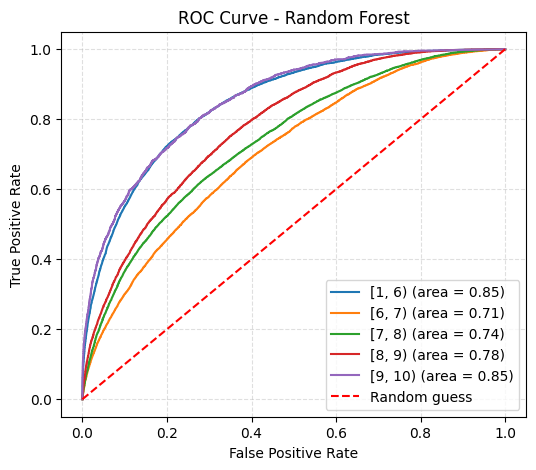
\includegraphics[width=\textwidth]{plotsss/roc_rf_rating}
        \caption{ROC Curve - Random Forest}
        \label{fig:roc_rf}
    \end{subfigure}
    \hfill
    \begin{subfigure}[b]{0.45\textwidth}
        \centering
        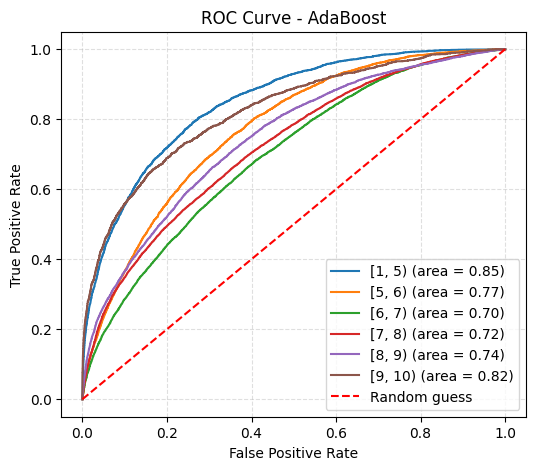
\includegraphics[width=\textwidth]{plotsss/roc_boost_rating}
        \caption{ROC Curve - AdaBoost}
        \label{fig:roc_ab}
    \end{subfigure}
    \caption{ROC curves for the ensemble models on the \texttt{averageRating} classification task.}
    \label{fig:roc_comparison}
\end{figure}
From these representations, it can be seen that AdaBoost has
poorer performances in all classes, but especially struggles
with the under-represented ones, which lead to the biggest
difference in Area Under The Curve (AUC).


On the \texttt{titleType} classification task, the best hyperparameters
obtained for the Random Forest model were:
% {'class_weight': None, 'criterion': 'gini', 'max_depth': 19, 'max_features': 0.7361716094628554, 'min_samples_leaf': 3, 'min_samples_split': 4, 'n_estimators': 42}
\texttt{n\_estimators=42}, \texttt{max\_depth=19}, \texttt{min\_samples\_split=4},
\texttt{min\_samples\_leaf=3}, \texttt{max\_features=0.74},
\texttt{criterion='gini'}, \texttt{class\_weight=None}.
% precision    recall  f1-score   support

%        movie       0.91      0.95      0.93     12947
%        short       0.93      0.96      0.95      4994
%    tvEpisode       0.96      0.98      0.97     21249
%     tvSeries       0.77      0.70      0.73      3247
%    tvSpecial       0.69      0.26      0.38       345
%        video       0.77      0.42      0.55      1545

%     accuracy                           0.92     44327
%    macro avg       0.84      0.71      0.75     44327
% weighted avg       0.92      0.92      0.92     44327


% adaboost
% Best parameters found for AdaBoost: {'estimator__max_depth': 10, 'estimator__min_samples_leaf': 16, 'estimator__min_samples_split': 16, 'learning_rate': 0.46606998421703594, 'n_estimators': 56}
For the AdaBoost model, the best hyperparameters were:
\texttt{n\_estimators=56}, \texttt{learning\_rate=0.47},
\texttt{estimator\_\_max\_depth=10},
\texttt{estimator\_\_min\_samples\_split=16},
\texttt{estimator\_\_min\_samples\_leaf=16}.
%            precision    recall  f1-score   support

%        movie       0.87      0.95      0.91     12947
%        short       0.92      0.95      0.94      4994
%    tvEpisode       0.96      0.97      0.96     21249
%     tvSeries       0.75      0.63      0.68      3247
%    tvSpecial       0.73      0.09      0.16       345
%        video       0.70      0.32      0.44      1545

The table below summarizes the classification report for both models.
\begin{table}[H]
    \centering
    \label{tab:classification_report}
    \begin{tabular}{lccccc}
    \hline
    \textbf{Model} & \textbf{Accuracy} & \textbf{Macro Precision} & \textbf{Macro Recall} & \textbf{Macro F1-score} \\
    \hline
    Random Forest & 0.92 & 0.84 & 0.71 & 0.75 \\
    AdaBoost & 0.90 & 0.82 & 0.65 & 0.68 \\
    \hline
    \end{tabular}
    \caption{Performances of the models on the \texttt{titleType} classification task.}
\end{table}

Figure~\ref{fig:cm_rf} and Figure~\ref{fig:cm_ab} show the confusion matrices
for the models.

\begin{figure}[H]
    \centering
    \begin{subfigure}[b]{0.49\textwidth}
        \centering
        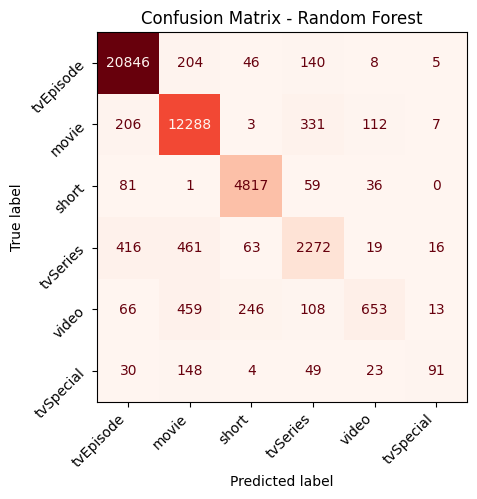
\includegraphics[width=\textwidth]{plotsss/conf_matr_rf_titletype}
        \caption{Confusion Matrix - Random Forest}
        \label{fig:cm_rf}
    \end{subfigure}
    \hfill
    \begin{subfigure}[b]{0.49\textwidth}
        \centering
        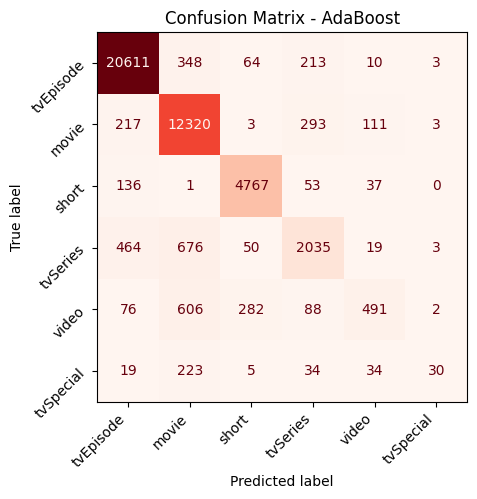
\includegraphics[width=\textwidth]{plotsss/conf_matr_boost_titletype}
        \caption{Confusion Matrix - AdaBoost}
        \label{fig:cm_ab}
    \end{subfigure}
    \caption{Confusion matrices for the ensemle models on the \texttt{titleType} classification task.}
    \label{fig:cm_comparison}
\end{figure}
Both models perform well on the first four classes, while struggling
with /texttt{video} and /texttt{tvSpecial}, which are the most
under-represented classes. In general, the two models show similar
performances, with Random Forest generally outperforming AdaBoost
by a slight margin.
Contrary to the results, the models base their decisions
on different feature importances: while Random Forest assigns over
half of the importance to \texttt{runtimeMinutes},
AdaBoost spreads the importance evenly across multiple features,
with the top being \texttt{runtimeMinutes} with around 15\%.


The ROC curves for the two models are shown in Figure~\ref{fig:roc_rf} and
Figure~\ref{fig:roc_ab}.
\begin{figure}[h]
    \centering
    \begin{subfigure}[b]{0.45\textwidth}
        \centering
        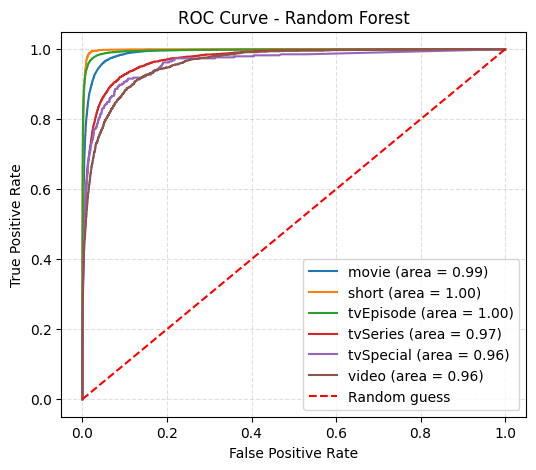
\includegraphics[width=\textwidth]{plotsss/roc_rf_titletype}
        \caption{ROC Curve - Random Forest}
        \label{fig:roc_rf}
    \end{subfigure}
    \hfill
    \begin{subfigure}[b]{0.45\textwidth}
        \centering
        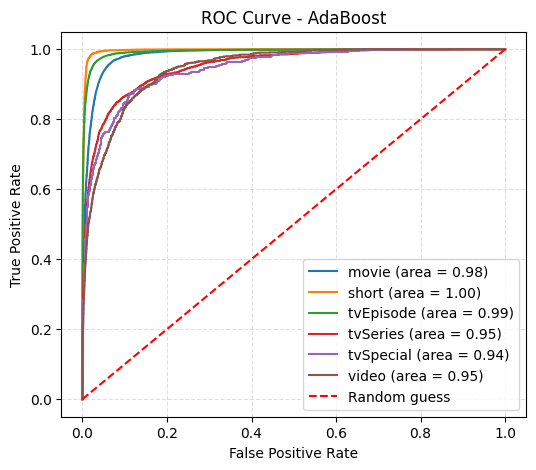
\includegraphics[width=\textwidth]{plotsss/roc_boost_titletype}
        \caption{ROC Curve - AdaBoost}
        \label{fig:roc_ab}
    \end{subfigure}
    \caption{ROC curves for the ensemble models on the \texttt{titleType} classification task.}
    \label{fig:roc_comparison}
\end{figure}

Again, similar performances are observed. The biggest difference
seems to be found in the under-represented classes, which seem to
have a bigger difference in Area Under The Curve (AUC).

\subsection{Neural Networks}


\subsection{Model Comparison}